\documentclass[usenames,dvipsnames,mathserif,notheorems]{beamer}

% silence annoying warnings
\usepackage{silence}
\usepackage{caption}
\WarningFilter{remreset}{The remreset package}
\usepackage{xcolor}
\usepackage{algorithm}
\usepackage{algorithmic}

%% Math macros for LaTex Projects 
%% Maintainer: Aaron Mishkin <amishkin@cs.stanford.edu>
%% Original Source: Mark Schmidt (UBC CS), Ben Bloem-Reddy (UBC Stats).

%% Easy bold-face 

\def\bfA{\mathbf{A}}
\def\bfB{\mathbf{B}}
\def\bfC{\mathbf{C}}
\def\bfD{\mathbf{D}}
\def\bfE{\mathbf{E}}
\def\bfF{\mathbf{F}}
\def\bfG{\mathbf{G}}
\def\bfH{\mathbf{H}}
\def\bfI{\mathbf{I}}
\def\bfJ{\mathbf{J}}
\def\bfK{\mathbf{K}}
\def\bfL{\mathbf{L}}
\def\bfM{\mathbf{M}}
\def\bfN{\mathbf{N}}
\def\bfO{\mathbf{O}}
\def\bfP{\mathbf{P}}
\def\bfQ{\mathbf{Q}}
\def\bfR{\mathbf{R}}
\def\bfS{\mathbf{S}}
\def\bfT{\mathbf{T}}
\def\bfU{\mathbf{U}}
\def\bfV{\mathbf{V}}
\def\bfW{\mathbf{W}}
\def\bfX{\mathbf{X}}
\def\bfY{\mathbf{Y}}
\def\bfZ{\mathbf{Z}}

% bb series
\def\bbA{\mathbb{A}}
\def\bbB{\mathbb{B}}
\def\bbC{\mathbb{C}}
\def\bbD{\mathbb{D}}
\def\bbE{\mathbb{E}}
\def\bbF{\mathbb{F}}
\def\bbG{\mathbb{G}}
\def\bbH{\mathbb{H}}
\def\bbI{\mathbb{I}}
\def\bbJ{\mathbb{J}}
\def\bbK{\mathbb{K}}
\def\bbL{\mathbb{L}}
\def\bbM{\mathbb{M}}
\def\bbN{\mathbb{N}}
\def\bbO{\mathbb{O}}
\def\bbP{\mathbb{P}}
\def\bbQ{\mathbb{Q}}
\def\bbR{\mathbb{R}}
\def\bbS{\mathbb{S}}
\def\bbT{\mathbb{T}}
\def\bbU{\mathbb{U}}
\def\bbV{\mathbb{V}}
\def\bbW{\mathbb{W}}
\def\bbX{\mathbb{X}}
\def\bbY{\mathbb{Y}}
\def\bbZ{\mathbb{Z}}

% cal series
\def\calA{\mathcal{A}}
\def\calB{\mathcal{B}}
\def\calC{\mathcal{C}}
\def\calD{\mathcal{D}}
\def\calE{\mathcal{E}}
\def\calF{\mathcal{F}}
\def\calG{\mathcal{G}}
\def\calH{\mathcal{H}}
\def\calI{\mathcal{I}}
\def\calJ{\mathcal{J}}
\def\calK{\mathcal{K}}
\def\calL{\mathcal{L}}
\def\calM{\mathcal{M}}
\def\calN{\mathcal{N}}
\def\calO{\mathcal{O}}
\def\calP{\mathcal{P}}
\def\calQ{\mathcal{Q}}
\def\calR{\mathcal{R}}
\def\calS{\mathcal{S}}
\def\calT{\mathcal{T}}
\def\calU{\mathcal{U}}
\def\calV{\mathcal{V}}
\def\calW{\mathcal{W}}
\def\calX{\mathcal{X}}
\def\calY{\mathcal{Y}}
\def\calZ{\mathcal{Z}}


%% Theorem Environments %%
\usepackage{amsthm}
\usepackage{thmtools, thm-restate}

\declaretheorem[numberwithin=section]{theorem}
\declaretheorem[numberwithin=section]{proposition}
\declaretheorem[numberwithin=section]{lemma}
\declaretheorem[numberwithin=section]{definition}
\declaretheorem[numberwithin=section]{assumption}
\declaretheorem[numberwithin=section]{corollary}
\declaretheorem[numberwithin=section]{example}
\declaretheorem[numbered=no]{remark}

%% Floor and Ceiling %%
\usepackage{mathtools} % required for \DeclarePairedDelimeter

%% Stochastic Relations %% 

% almost sure:
\newcommand{\as}[1]{\stackrel{\text{\rm\tiny a.s.}}{#1}}
% a.s.\ equality:
\newcommand{\equas}{\stackrel{\text{\rm\tiny a.s.}}{=}}

% in distribution:
\newcommand{\dist}[1]{\stackrel{\text{\rm\tiny dist}}{#1}}
% equality in distribution:
\newcommand{\equdist}{\stackrel{\text{\rm\tiny dist}}{=}}

% independent
\newcommand{\ind}[0]{\perp \!\!\! \perp }

%% Variance, Expectation, etc %%
\newcommand{\Var}[1]{\textbf{Var}\sbr{#1}}

% ceiling and floor
\DeclarePairedDelimiter{\ceil}{\lceil}{\rceil}
\DeclarePairedDelimiter{\floor}{\lfloor}{\rfloor}
\newcommand{\argdot}{{\,\vcenter{\hbox{\tiny$\bullet$}}\,}} %generic argument dot

% absolute value
\newcommand{\abs}[1]{\left\vert #1\right\vert}

\newcommand{\seq}[1]{\rbr{#1}}

% easy bracketing:
\newcommand{\rbr}[1]{\left(#1\right)}
\newcommand{\sbr}[1]{\left[#1\right]}
\newcommand{\cbr}[1]{\left\{#1\right\}}
\newcommand{\abr}[1]{\left\langle#1\right\rangle}

% Norms
\def\norm#1{\|#1\|}
\def\biggnorm#1{\bigg\|#1\bigg\|}
% Random Variable Norms:
\def\psitwo#1{\|#1\|_{\psi_2}}
\def\psione#1{\|#1\|_{\psi_1}}

% mid
\newcommand{\biggmid}{\bigg \vert }

% argmax/argmin
\def\argmax{\mathop{\rm arg\,max}}
\def\argmin{\mathop{\rm arg\,min}}

% General Symbols
\def\half{\frac 1 2}
\newcommand{\inv}[1]{\frac{1}{#1}}
\newcommand{\halved}[1]{\frac{#1}{2}}
\newcommand{\R}{\mathbb{R}}
\newcommand{\eR}{\bar{\mathbb{R}}}

\newcommand{\into}{\rightarrow}

% Gradient Descent Symbols
\newcommand{\oracle}{\mbox{\( \calO \)}}
\newcommand{\iter}{k}

\newcommand{\Lk}{L_{\zk}}
\newcommand{\Lmax}{L_{\text{max}}}
\newcommand{\mumax}{\mu_{\text{max}}}
\newcommand{\Lmin}{L_{\text{min}}}
\newcommand{\mumin}{\mu_{\text{min}}}

% iterates
\newcommand{\y}{y}
\newcommand{\yk}{y_k}
\newcommand{\ykk}{y_{k+1}}

\newcommand{\vk}{v_k}
\newcommand{\vkk}{v_{k+1}}

\newcommand{\w}{w}
\newcommand{\wk}{w_k}
\newcommand{\wkk}{w_{k+1}}
\newcommand{\wopt}{w^*}
\newcommand{\wbar}{\bar{w}}


\newcommand{\x}{x}
\newcommand{\xk}{x_k}
\newcommand{\xkplus}{x_k^+}
\newcommand{\xkk}{x_{k+1}}
\newcommand{\xopt}{x^*}
\newcommand{\xbar}{\xbar{w}}

% noise
\newcommand{\Z}{Z}
\newcommand{\z}{z}
\newcommand{\zk}{z_{k}}
\newcommand{\zkk}{z_{k+1}}
% step-sizes
\newcommand{\tetak}{{\tilde{\eta}}_{k}}
\newcommand{\etamin}{\eta_{\text{min}}}
\newcommand{\etamax}{\eta_{\text{max}}}
\newcommand{\etak}{\eta_k}
\newcommand{\etakk}{\eta_{k+1}}

\newcommand{\betak}{\beta_{k}}
\newcommand{\betakk}{\beta_{k+1}}
\newcommand{\alphak}{\alpha_{k}}
\newcommand{\alphakk}{\alpha_{k+1}}

\newcommand{\Ek}{\bbE_{\zk}}
\newcommand{\E}{\bbE}

% functions
\newcommand{\f}{f}
\newcommand{\fj}{f_i}
\newcommand{\fopt}{f^*}
% sub-sampled functions
\newcommand{\fk}{f_{i_k}}
\newcommand{\fkk}{f_{i_{(k+1)}}}
% gradients
\newcommand{\grad}{\nabla f}
% sub-sampled gradients
\newcommand{\gradk}{\nabla f_{i_k}}
\newcommand{\gradkk}{\nabla f_{i_{(k+1)}}}

%% Weak and strong growth constants
\newcommand{\sgc}{\rho}
\newcommand{\wgc}{\alpha}
%%%%%%%%%%%%%%%%%%%%%%%%%%%%%%%%%%%%%%%%%%%%%%%%%%%%%%%%%%


%% Etc %%  

%% add numbers to align* environments.
\newcommand{\addnumber}{\addtocounter{equation}{1}\tag{\theequation}}

%%%%%%%%%


%% Group Lasso %%
\newcommand{\bi}{{b_i}}
\newcommand{\wi}{w_\bi}
\newcommand{\vi}{v_\bi}
\newcommand{\zi}{z_\bi}
\newcommand{\Xbi}{X_\bi}
\newcommand{\act}{{\calA_{\lambda}}}
\newcommand{\inact}{{\calI_{\lambda}}}
\newcommand{\tran}{{\calT_{\lambda}}}
\newcommand{\equi}{{\calE_{\lambda}}}

\newcommand{\acts}{{\calA_{\lambda}^{*}}}
\newcommand{\trans}{{\calT_{\lambda}^{*}}}

\newcommand{\wa}{w_\act}
\newcommand{\was}{w_\acts}
\newcommand{\we}{w_\equi}
\newcommand{\va}{v_\act}
\newcommand{\vas}{v_\acts}
\newcommand{\ve}{v_\equi}
\newcommand{\Xa}{X_\act}
\newcommand{\Xas}{X_\acts}
\newcommand{\Xe}{X_\equi}

\newcommand{\wmin}{w^*}
\newcommand{\solfn}{\calW^*}

\newcommand{\Null}{\text{Null}}
\newcommand{\Row}{\text{Row}}
\newcommand{\Span}{\text{Span}}

%% Plotting macros for LaTex Projects 
%% Maintainer: Aaron Mishkin <amishkin@cs.stanford.edu>


%% Tikz and PGFplots packages
\usepackage{tikz}
\usepackage{pgfplots}

% tikz and PGFplots libraries
\usepgfplotslibrary{fillbetween}
\usetikzlibrary{patterns}



%% tikz settings 
\tikzset{
    font={\fontsize{12pt}{12}\selectfont},
}

%% PGFplots settings 
\pgfplotsset{
    % version compatibility
    compat=1.5.1,
    % basic line-styles
    primary/.style={color=black, style=solid, line width=1.5pt}, 
    secondary/.style={color=red, style=solid, line width=1.5pt}, 
}


\usetikzlibrary{shapes, decorations.pathreplacing,calligraphy}

\usepackage{simplebeam}
\usetheme{simplebeamer}

% bib resources
\addbibresource[]{refs.bib}

\title{The Solution Path of the Group Lasso}
\subtitle{}
\author{Aaron Mishkin \and Mert Pilanci}
\institute{Stanford University}
\collaborators{
	
\includegraphics[width=0.2\linewidth]{assets/aaron.png}
	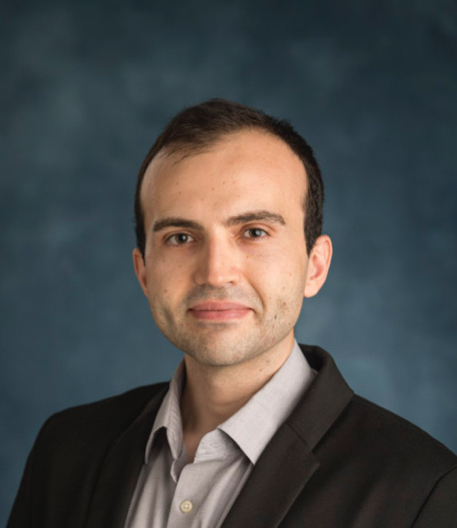
\includegraphics[width=0.2\linewidth]{assets/mert.jpg}
}

\titlegraphic{
\includegraphics[width=0.4\textwidth]{assets/stanford.eps}}

\newcommand{\horizontalrule}{
	{
			\vspace{-0.5em}
			\center \rule{\textwidth}{0.1em}
			\vspace{-0.2em}
		}
}

\newcommand{\red}[1]{\textcolor{Red}{#1}}
\newcommand{\green}[1]{\textcolor{ForestGreen}{#1}}
\newcommand{\blue}[1]{\textcolor{DarkBlue}{#1}}
\newcommand{\purple}[1]{\textcolor{Magenta}{#1}}

%\logo{\includegraphics[height=0.5cm]{assets/Block_S_2_color.eps}}

%\institute{Stanford University}
\date{}

\begin{document}

\maketitle

%% main content starts %%
\begin{frame}{Intro: Contributions}
	\red{Problem}: Continuity of the group Lasso solution path is unknown.
	\pause
	\begin{itemize}
		\item \textbf{Non-linear}: Unlike the classical lasso, the group Lasso path is non-linear \citep{efron2004least}.
		      \pause
		\item \textbf{Uniqueness}: The optimal solution is not unique in general.
		      \pause
		\item \textbf{Break Points}: There can be countably many potential discontinuities to check.
	\end{itemize}
	\pause
	\horizontalrule

	\green{Our Contributions}:
	\begin{itemize}
		\pause
		\item We characterize the \textbf{optimal set} for the group lasso under general conditions.
		      \pause
		\item We establish \textbf{weaker sufficient conditions} for the solution to be unique.
		      \pause
		\item We prove \textbf{continuity} of the unique solution path.
	\end{itemize}
\end{frame}


\begin{frame}{Intro: Problem Setup}
	\textbf{Problem Setup}:
	\begin{itemize}
		\item \( X \in \R^{n \times d} \) is a design matrix with associated targets \( y \in \R^n \).
		\item \( \calB = \cbr{b_1, \ldots b_m} \) is a partition of the features.
		\item \( \lambda \geq 0 \) controls the regularization strength.
	\end{itemize}

	\vspace{0.5em}
	\pause

	The \green{solution path} of the Group Lasso is given by
	\[
		\calW^*(\lambda) = \argmin_{w} \half \norm{X w - y}_2^2 + \lambda \sum_{\bi \in \calB} \norm{\wi}_2
	\]

	\horizontalrule
	\pause

	\red{Problem}: when is \( \lambda \mapsto \calW^*(\lambda) \) single-valued and continuous?

\end{frame}


\begin{frame}{Intro: the Importance of Continuity}

	Consider the problem of minimizing the validation error,
	\[
		\calV(\lambda) = \min_{w^* \in \calW^*(\lambda)} \norm{\tilde X w^* - \tilde y}_2^2.
	\]

	\pause

	\begin{figure}[]
		\centering
		%! TEX root = ../main.tex

%% Illustration of cone decomposition. 

\begin{tikzpicture}[scale=1,
		declare function={
				cv(\x) = ((abs(\x)^3) / 4 - \x^2/2 + \x/2);
				gmin(\x) = 10*(\x - 1)^2 - 2;
			}
	]
	\begin{axis}[width=1.1\linewidth, height=6cm,
			axis lines=center, yticklabels={,,}, xticklabels={,,},
			ymin=-4, ymax=4, ytick={-5,...,5}, ylabel=$$, x axis line style={-},
				xmin=-6, xmax=6, xtick={-5,...,5}, xlabel=$$, y axis line style={-},
		]
		% function
		\addplot[name path=cv_left, domain=-6:0.8, samples=100, line width=1pt]{cv(x)};
		\addplot[name path=cv_right, domain=1.2:6, samples=100, line width=1pt]{cv(x)};

		%% discontinuity
		\addplot[name path=cv_discont, domain=0.8:1.2, samples=10, line width=1pt]{gmin(x)};
		%\addplot +[mark=none, line width=1pt, dashed, draw=red] coordinates {(0.8, -1.85) (0.8, 0.22)};
		%\addplot +[mark=none, line width=1pt, dashed, draw=red] coordinates {(1.2, -1.85) (1.2, 0.322)};



		\addplot +[mark=none, line width=1pt, dashed, draw=blue] coordinates {(0.8, 0.322) (0.8, 1.36)};
		\addplot +[mark=none, line width=1pt, dashed, draw=blue] coordinates {(1.2, 0.322) (1.2, 1.36)};

		\node [circle, fill=white, inner sep=1.2pt, draw=black, line width=1pt] at (axis cs:0.8, 0.22) {};
		\node [circle, fill=white, inner sep=1.2pt, draw=black, line width=1pt] at (axis cs:1.2, 0.322) {};

		\node [circle, fill=black, inner sep=1.0pt] at (axis cs:0.8, -1.6) {};
		\node [circle, fill=black, inner sep=1.0pt] at (axis cs:1.2, -1.6) {};

		% epsilon net 
		%\addplot [name path=cv_left, domain=-4:0.5, samples=8, only marks, mark=|, fill=blue, draw=blue, mark size=5, line width=1]{cv(x)};

		%\addplot [name path=cv_left, domain=1.5:5, samples=7, only marks, mark=|, fill=blue, draw=blue, mark size=5, line width=1]{cv(x)};

		% labels

		\node[label={270:$\lambda^*$}, circle, fill=red, inner sep=1.4pt] (opt) at (axis cs:1, -2) {};

		\node[label={270:$\calV(\lambda)$}] at (axis cs:-2.4, 3) {};

		\draw [decorate, decoration = {calligraphic brace}, line width=1.2pt] (axis cs:0.8, 1.43) --  (axis cs:1.2, 1.43);

		\node[label={90:$\epsilon$}] at (axis cs:1.0, 1.41) {};
	\end{axis}

\end{tikzpicture}%

	\end{figure}

\end{frame}

\begin{frame}{Intro: the Importance of Continuity}

	Consider the problem of minimizing the validation error,
	\[
		\calV(\lambda) = \min_{w^* \in \calW^*(\lambda)} \norm{\tilde X w^* - \tilde y}_2^2.
	\]

	\begin{figure}[]
		\centering
		%! TEX root = ../main.tex

%% Illustration of cone decomposition. 

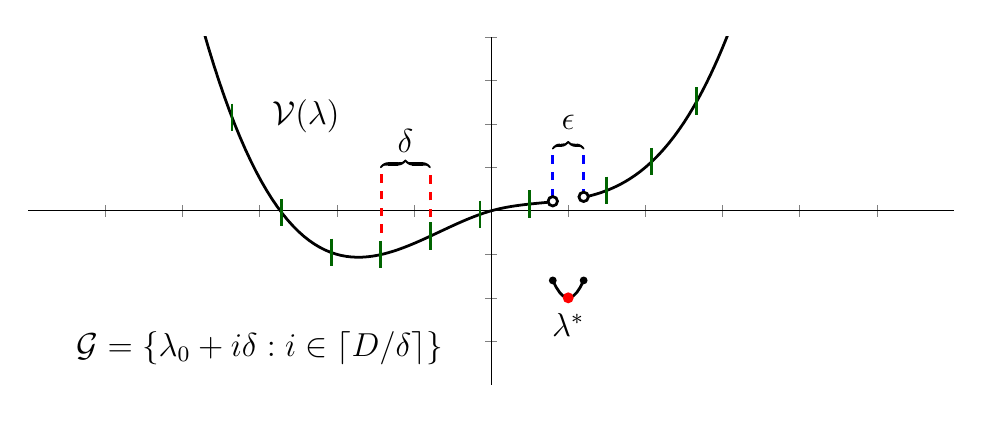
\begin{tikzpicture}[scale=1,
		declare function={
				cv(\x) = ((abs(\x)^3) / 4 - \x^2/2 + \x/2);
				gmin(\x) = 10*(\x - 1)^2 - 2;
			}
	]
	\begin{axis}[width=1.1\linewidth, height=6cm,
			axis lines=center, yticklabels={,,}, xticklabels={,,},
			ymin=-4, ymax=4, ytick={-5,...,5}, ylabel=$$, x axis line style={-},
				xmin=-6, xmax=6, xtick={-5,...,5}, xlabel=$$, y axis line style={-},
		]
		% function
		\addplot[name path=cv_left, domain=-6:0.8, samples=100, line width=1pt]{cv(x)};
		\addplot[name path=cv_right, domain=1.2:6, samples=100, line width=1pt]{cv(x)};

		%% discontinuity
		\addplot[name path=cv_discont, domain=0.8:1.2, samples=10, line width=1pt]{gmin(x)};

		\addplot +[mark=none, line width=1pt, dashed, draw=blue] coordinates {(0.8, 0.322) (0.8, 1.36)};
		\addplot +[mark=none, line width=1pt, dashed, draw=blue] coordinates {(1.2, 0.322) (1.2, 1.36)};

		\node [circle, fill=white, inner sep=1.2pt, draw=black, line width=1pt] at (axis cs:0.8, 0.22) {};
		\node [circle, fill=white, inner sep=1.2pt, draw=black, line width=1pt] at (axis cs:1.2, 0.322) {};

		\node [circle, fill=black, inner sep=1.0pt] at (axis cs:0.8, -1.6) {};
		\node [circle, fill=black, inner sep=1.0pt] at (axis cs:1.2, -1.6) {};


		% epsilon net 
		\addplot [name path=cv_left, domain=-4:0.5, samples=8, only marks, mark=|, fill=blue, draw=DarkGreen, mark size=5, line width=1]{cv(x)};

		\addplot [name path=cv_left, domain=1.5:5, samples=7, only marks, mark=|, fill=blue, draw=DarkGreen, mark size=5, line width=1]{cv(x)};

		% labels

		\node[label={270:$\lambda^*$}, circle, fill=red, inner sep=1.4pt] (opt) at (axis cs:1, -2) {};

		\node[label={270:$\calV(\lambda)$}] at (axis cs:-2.4, 3) {};

		\draw [decorate, decoration = {calligraphic brace}, line width=1.2pt] (axis cs:0.8, 1.43) --  (axis cs:1.2, 1.43);

		\node[label={90:$\epsilon$}] at (axis cs:1.0, 1.41) {};

		\addplot +[mark=none, line width=1pt, dashed, draw=red] coordinates {(-1.425, -0.5) (-1.425, 1.0)};
		\addplot +[mark=none, line width=1pt, dashed, draw=red] coordinates {(-0.787, -0.14) (-0.787, 1.0)};

		\draw [decorate, decoration = {calligraphic brace}, line width=1.2pt] (axis cs:-1.43, 1.0) --  (axis cs:-0.792, 1.0);

		\node[label={90:$\delta$}] at (axis cs:-1.111, 0.9) {};

		\node[label={$\calG = \cbr{\lambda_0 + i \delta : i \in \ceil{D / \delta}}$}] at (axis cs:-3.0, -4.0) {};
	\end{axis}

\end{tikzpicture}%

	\end{figure}

	\pause
	We must have \( \delta < \epsilon \),
	which can be \red{arbitrarily small}!

\end{frame}


\begin{frame}{Main Challenge: Non-Linear Solution Paths}

	\begin{columns}
		\begin{column}{0.5\textwidth}
			\centering
			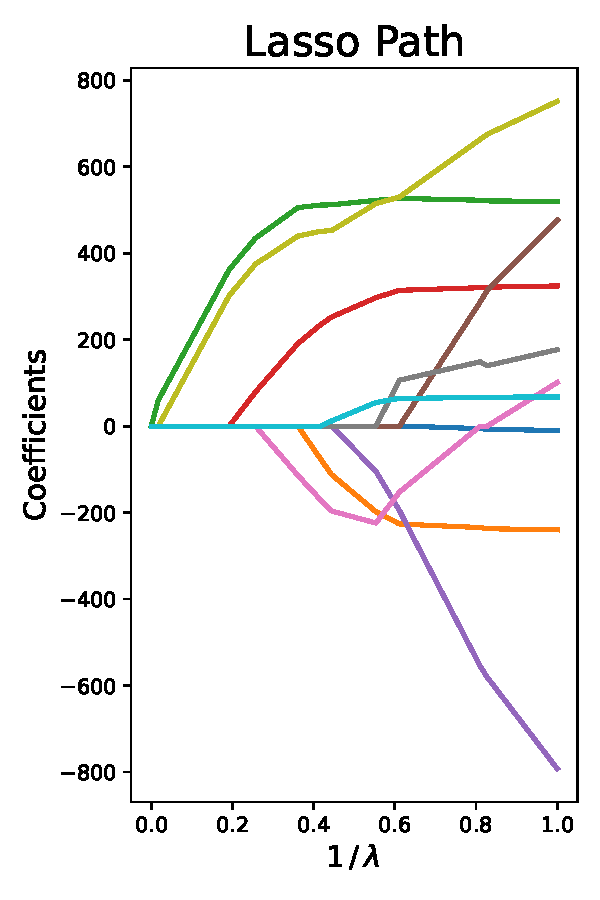
\includegraphics[width=\textwidth]{assets/lasso_path.pdf}
		\end{column}
		\pause
		\begin{column}{0.5\textwidth}
			\centering
			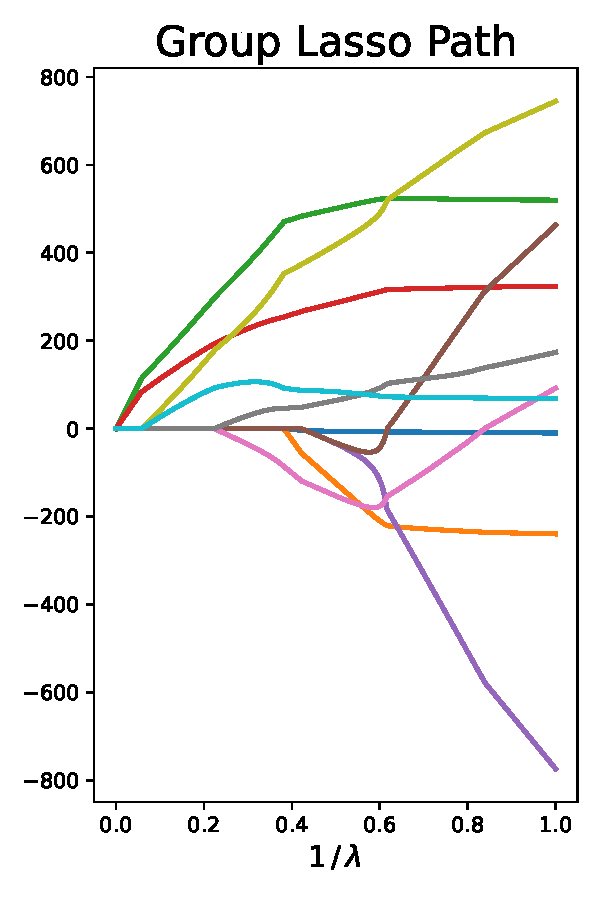
\includegraphics[width=\textwidth]{assets/group_lasso_path.pdf}
		\end{column}
	\end{columns}

\end{frame}


\begin{frame}{Analysis: Equicorrelation Set}
	\[
		\textbf{Group Lasso}: \calW^*(\lambda) = \argmin_{w} \half \norm{X w - y}_2^2 + \lambda \sum_{\bi \in \calB} \norm{\wi}_2
	\]
	\pause
	\horizontalrule

	First-order optimality conditions are
	\begin{equation*}\label{eq:fo-optimality}
		\blue{\Xbi^\top} \red{(y - X w)} \in
		\begin{cases}
			\cbr{\lambda \frac{\wi}{\norm{\wi}_2}} & \mbox{if \( \wi \neq 0 \)} \\
			\cbr{v : \norm{v}_2 \leq \lambda }     & \mbox{otherwise,}
		\end{cases}
	\end{equation*}

	\pause

	The \textbf{equicorrelation set} contains all non-zero blocks:
	\begin{equation}\label{eq:equi}
		\equi := \cbr{\bi \in \calB : \norm{\blue{\Xbi^\top} \red{(y - Xw)}}_2 = \lambda},
	\end{equation}


\end{frame}

\begin{frame}{Analysis: Optimal Set}
	Define the block-correlation vectors,
	\[
		\vi = \blue{\Xbi^\top} \red{(y - X w)}.
	\]
	and let \( w^* \in \solfn(\lambda) \) be the min-norm solution.
	Define
	\[
		\calN_\lambda = \Null(\Xe) \bigcap \cbr{z : \zi \in \Span(\vi), i \in \equi }.
	\]
	\vspace{-2em}
	\pause
	\begin{proposition}
		Let \( \lambda > 0 \).
		The optimal set is given by
		\[
			\begin{aligned}
				\solfn(\lambda) =
				\big\{
				w \in \R^d : \red{\we = \wmin_\equi(\lambda) + z,
					z \in \calN_\lambda}, \,
				w_{\inact} = 0, \, \\
				\wi \neq 0 \implies \frac{\lambda \wi}{\norm{\wi}_2} = \vi(\lambda)
				\big\}.
			\end{aligned}
		\]
	\end{proposition}

	\pause

	The solution is \green{unique} when \( \calN_{\lambda} = \cbr{0} \).

\end{frame}

\begin{frame}{Analysis: Conditions for Uniqueness}

	\textbf{Idea}: Study unique case by working backwards from \( \calN_\lambda = \cbr{0} \).

	\vspace{1em}
	\pause

	\begin{beamercolorbox}[wd=\textwidth,sep=1em]{relaxation}
		Assumption (Group General Position)

		For every \( \calE \subseteq \calB \), \( \abs{\calE} \leq n +1 \),
		there do not exist unit vectors \( \zi \in \R^{\abs{\bi}} \)
		such that for any \( j \in \calE \),
		\[
			X_{b_j} z_{b_j} \in
			\text{affine}(\cbr{\Xbi \zi : \bi \in \calE \setminus b_j}).
		\]
	\end{beamercolorbox}
	\vspace{1em}
	\pause

	\begin{itemize}
		\item Group general position extends the classical notion of general
		      position, which is sufficient for uniqueness of the lasso \citep{tibshirani2013unique}.
		      \pause

		\item We formally prove group general position is \green{sufficient} for the
		      group lasso to be unique.
	\end{itemize}

\end{frame}


\begin{frame}{Analysis: Continuity of the Solution Path}

	\begin{columns}
		\begin{column}{0.5\textwidth}
			\centering
			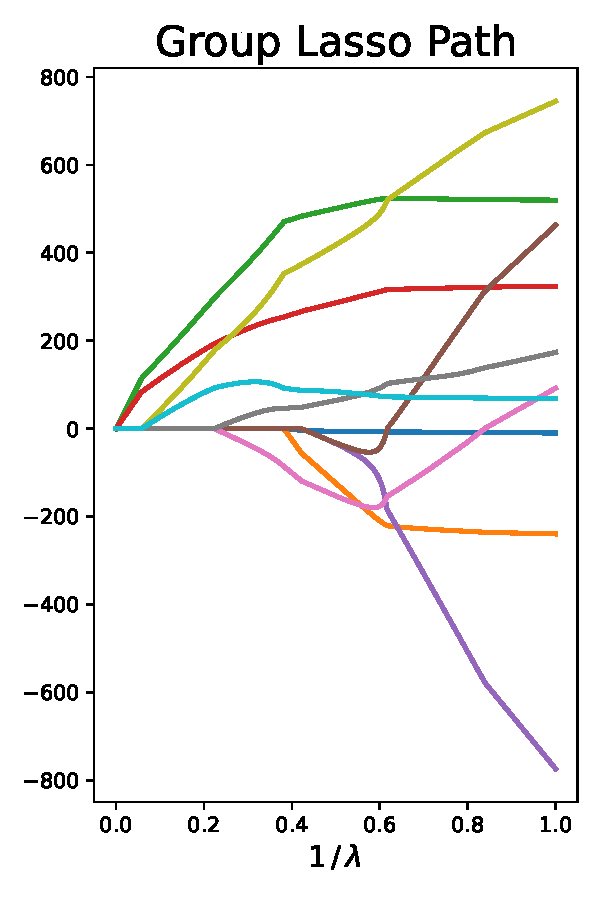
\includegraphics[width=\textwidth]{assets/group_lasso_path.pdf}
		\end{column}
		\begin{column}{0.5\textwidth}
			\textbf{Proof Strategy}:
			\begin{enumerate}
				\pause
				\item Establish continuity between breakpoints using
				      the implicit function theorem.
				      \pause
				\item Show left and right limits at each break point
				      are also solutions.
				      \pause
				\item Leverage uniqueness to deduce the left and right limits
				      are equal.
			\end{enumerate}
			\pause
			\begin{theorem}
				Suppose group general position holds.
				Then the unique group lasso solution path is continuous.
			\end{theorem}
		\end{column}
	\end{columns}
\end{frame}

%% main content ends %%

%% end slide
\setbeamercolor{background canvas}{bg=LightCyan}

\begin{frame}{}
	\begin{center}
		\huge Thanks for Listening!
	\end{center}
\end{frame}
\setbeamercolor{background canvas}{bg=white}

%% bibliography
\begin{frame}[allowframebreaks]{References}
	\printbibliography[]
\end{frame}


\end{document}
